\section{多组学简介}
\begin{frame}
  \frametitle{多组学 | 中心法则}
\begin{columns}
    \column{0.3\textwidth}
      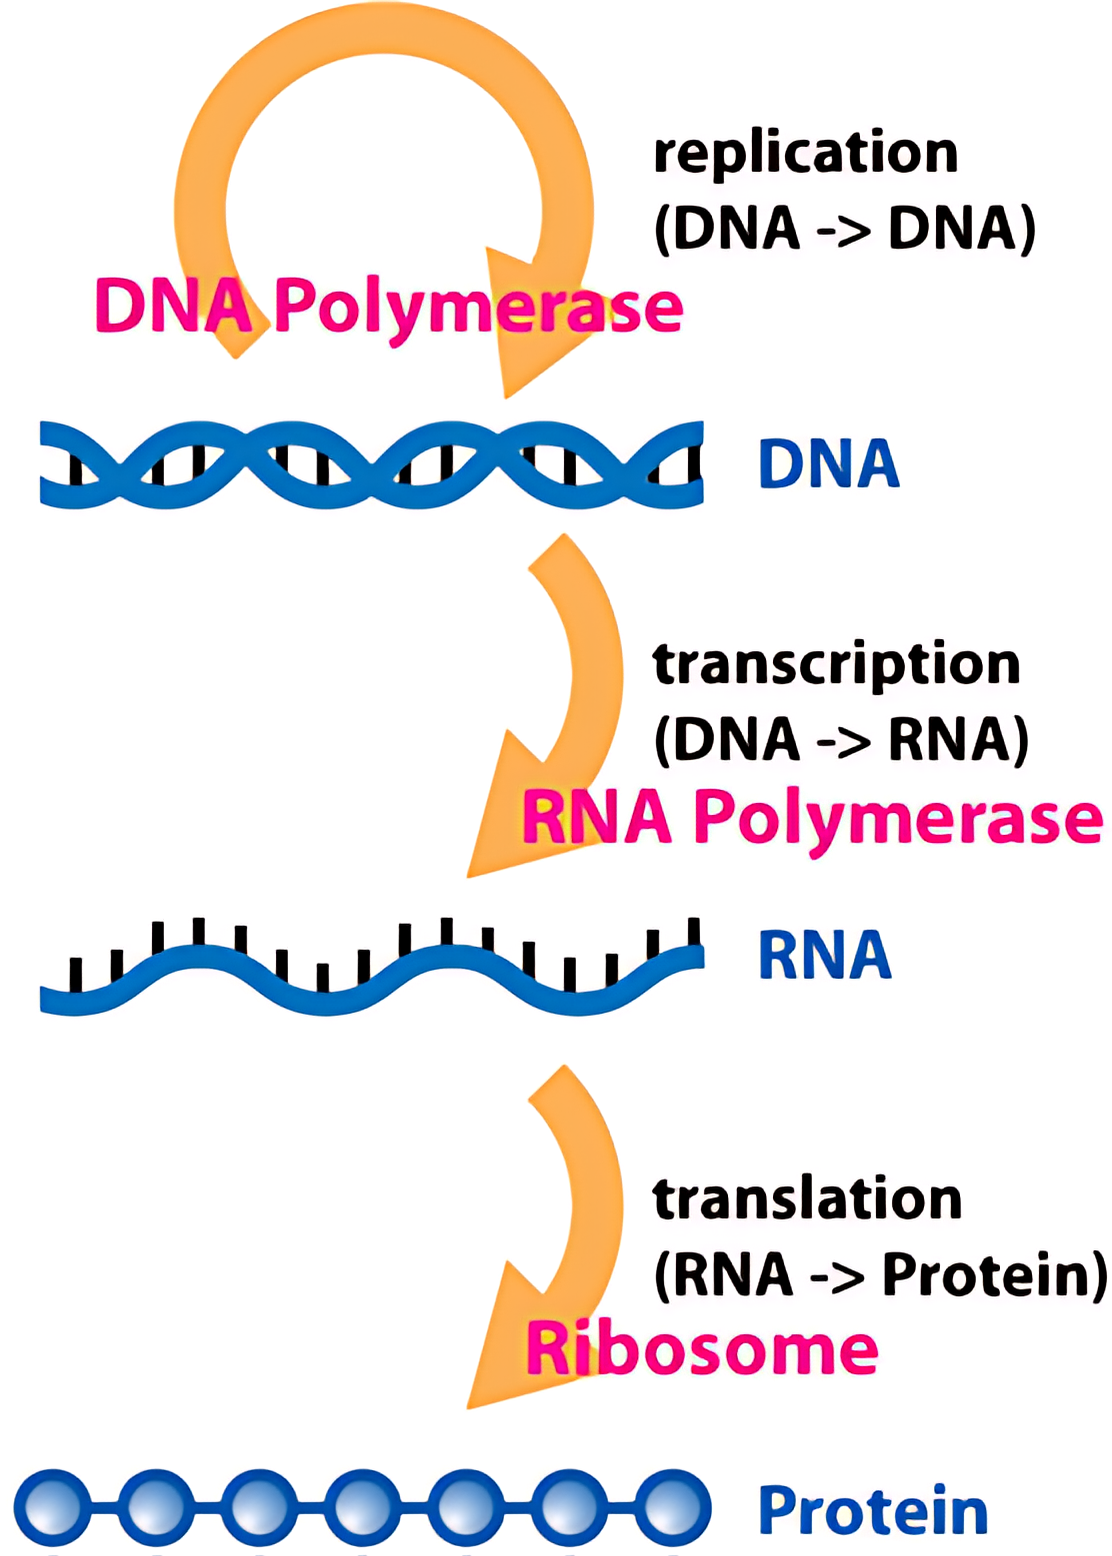
\includegraphics[width=\textwidth]{figures/c1_multiomics/dogma.png}
      \pause
    \column{0.2\textwidth}
    \begin{block}{生物分子}
        \begin{itemize}
            \item DNA
            \item RNA
            \item 蛋白质
            \item 糖
            \item 脂
            \item 代谢物
            \item ……
        \end{itemize}
    \end{block}
      \pause
    \column{0.38\textwidth}
    \begin{block}{生物分子的修饰（表观）}
        \begin{itemize}
            \item DNA修饰（DNA甲基化、组蛋白修饰）
            \item DNA三维结构
            \item RNA修饰（m6A、m1A、m5C）
            \item 翻译后修饰（磷酸化、乙酰化、泛素化）
            \item ……
        \end{itemize}
    \end{block}
    \end{columns}
\end{frame}

\begin{frame}
  \frametitle{多组学 | 组学}
\begin{columns}
    \column{0.5\textwidth}
      
\includegraphics[width=\textwidth]{figures/c1_multiomics/omics.png}
    \column{0.4\textwidth}
    \begin{block}{组学}
        \alert{组学（Omics）} 通常指生物学中对各类研究对象（一般为生物分子）的集合所进行的系统性研究，例如基因组学、蛋白质组学和代谢物组学等。
    \end{block}
    \begin{block}{组}
        这些研究对象的集合被称为组。
    \end{block}
\end{columns}
\end{frame}

\begin{frame}
  \frametitle{多组学 | 组学技术}
  \begin{figure}
    \centering
    \includegraphics[width=\textwidth]{figures/c1_multiomics/techs.png}
  \end{figure}
\end{frame}

\begin{frame}
  \frametitle{多组学 | 多组学简介}
  \begin{figure}
    \centering
    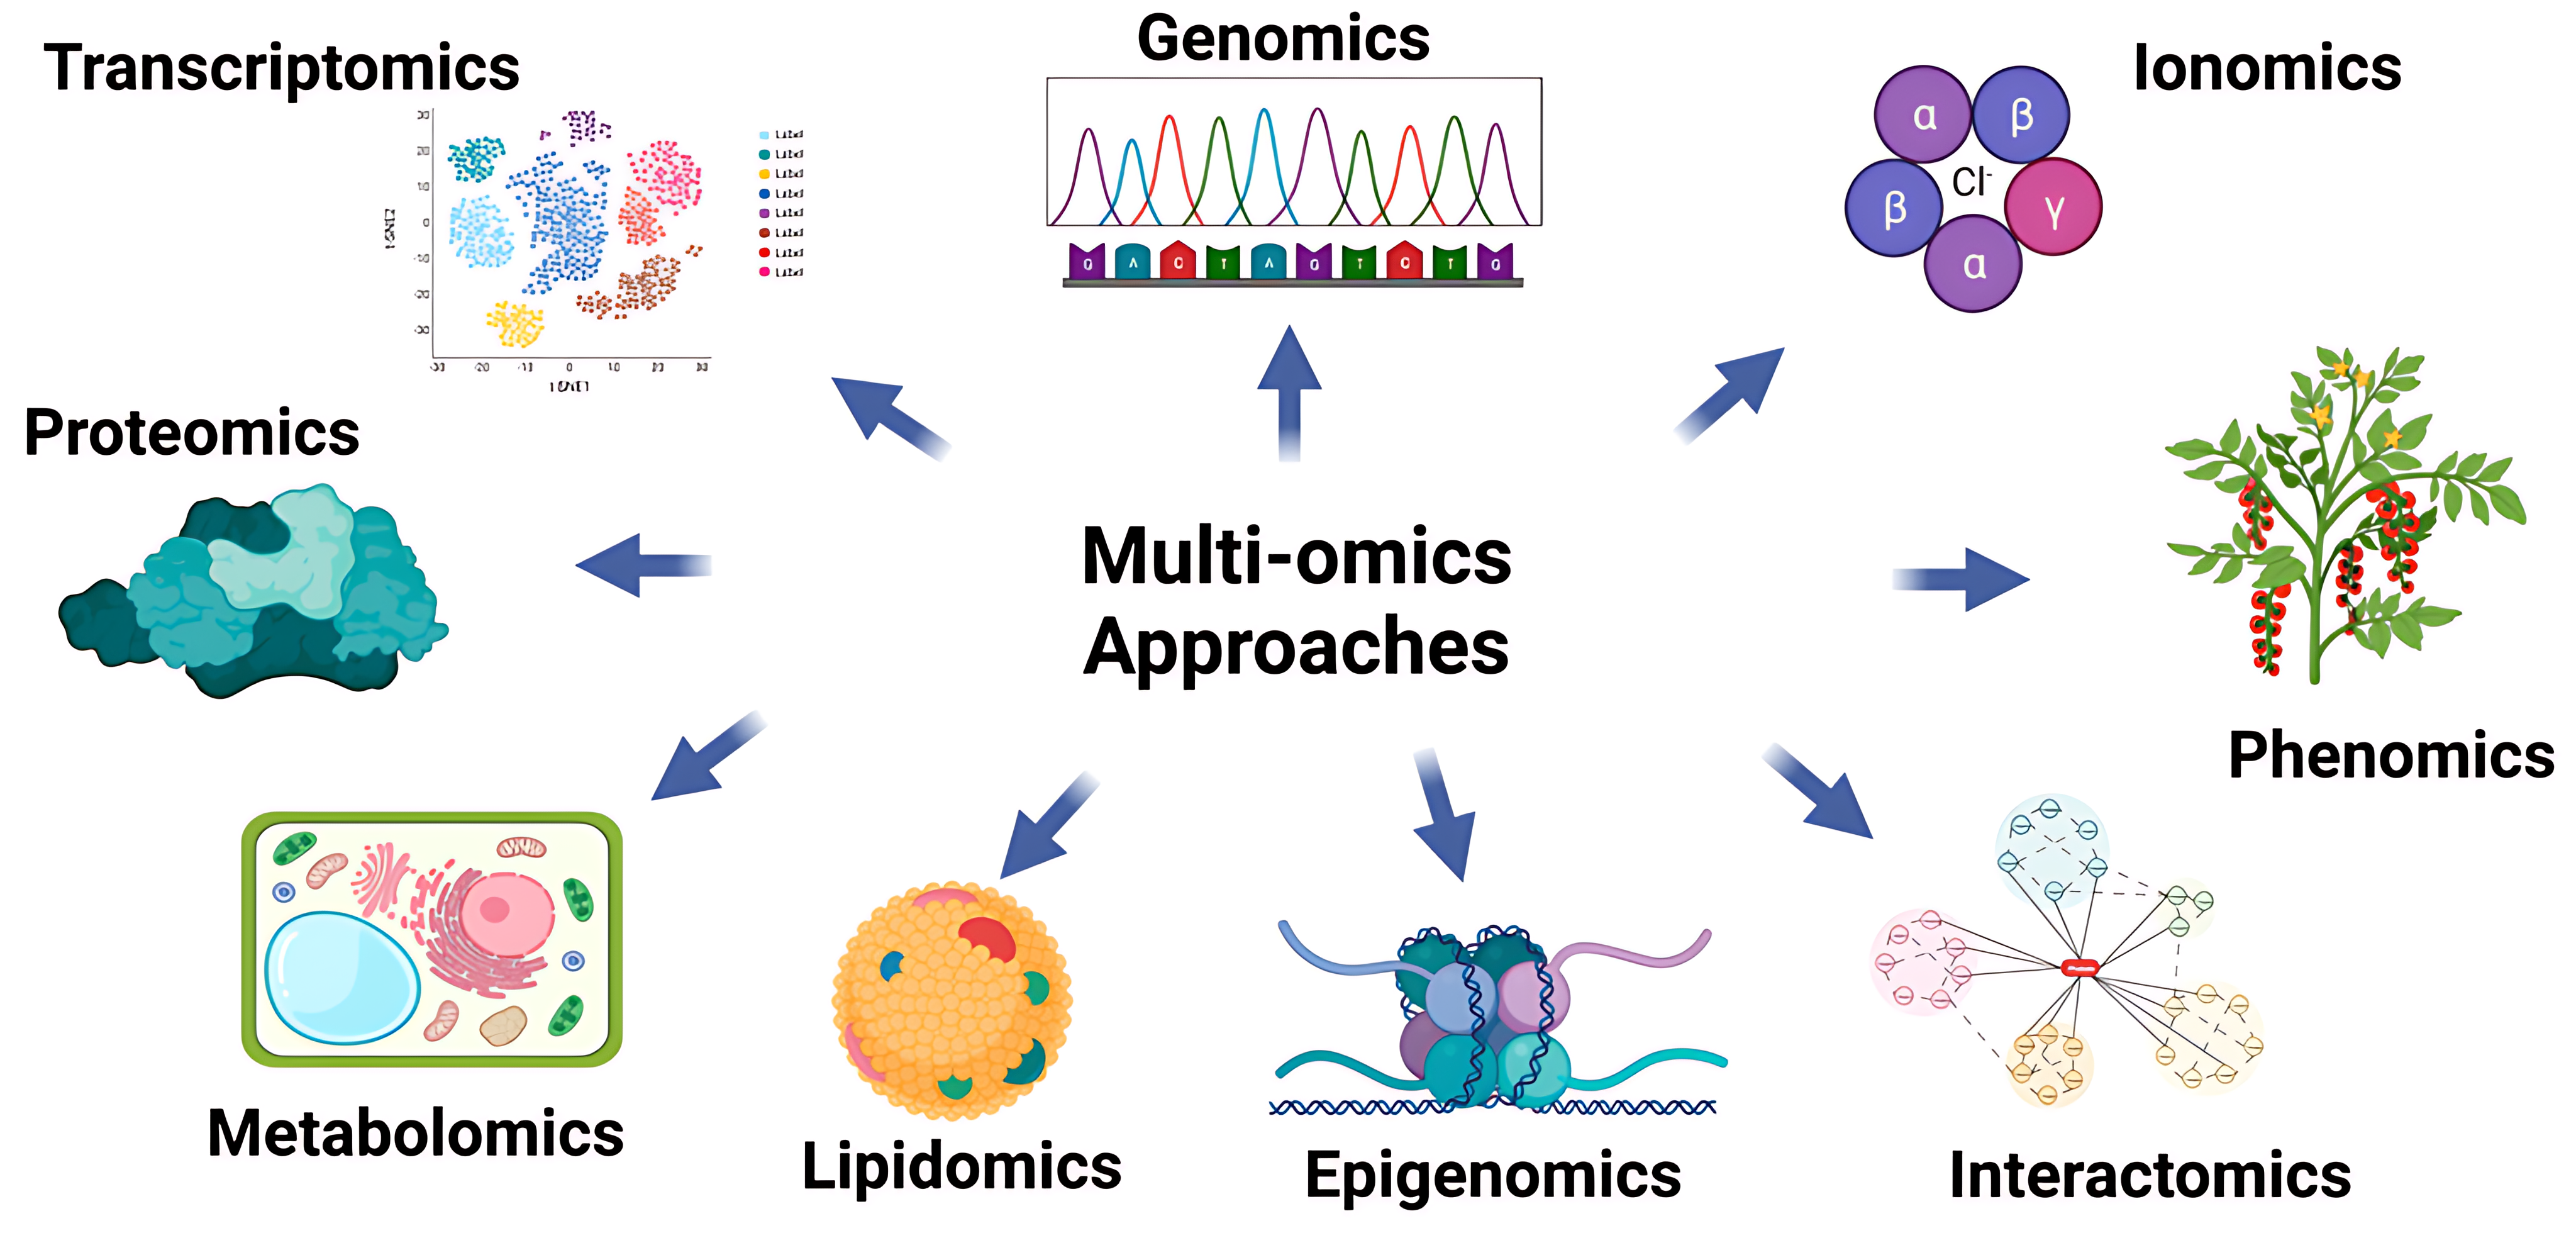
\includegraphics[width=\textwidth]{figures/c1_multiomics/multiomics.png}
  \end{figure}
\end{frame}

\begin{frame}
  \frametitle{多组学 | 多组学简介}
  \begin{block}{多组学}
      \alert{多组学（Multiomics）} 是对多重数据（包括基因组、表观基因组、蛋白质组、代谢物组、暴露组和微生物组等）的生物学分析方法；换言之就是用多组学技术一致性研究生命。
  \end{block}
  \begin{block}{多组学研究意义}
     \begin{itemize}
         \item 生命体是一个复杂的调控系统，疾病的发生与发展涉及到基因组、转录组、表观组、蛋白组及代谢组等多个不同层次的病理过程。
         \item 多组学分析研究能够帮助研究人员更好地将基因型与表型联系起来，更全面地了解分子变化对正常发育、细胞响应和疾病的影响。
     \end{itemize} 
  \end{block}
\end{frame}

\begin{frame}
  \frametitle{多组学 | 多组学简介}
  \begin{figure}
    \centering
    
\includegraphics[width=\textwidth]{figures/c1_multiomics/disease.png}
  \end{figure}
\end{frame}

\begin{frame}
  \frametitle{多组学 | 多组学简介}
  \begin{figure}
    \centering
    \includegraphics[width=\textwidth]{figures/c1_multiomics/vs.png}
  \end{figure}
\end{frame}

\begin{frame}
  \frametitle{多组学 | 多组学简介}
  \begin{figure}
    \centering
    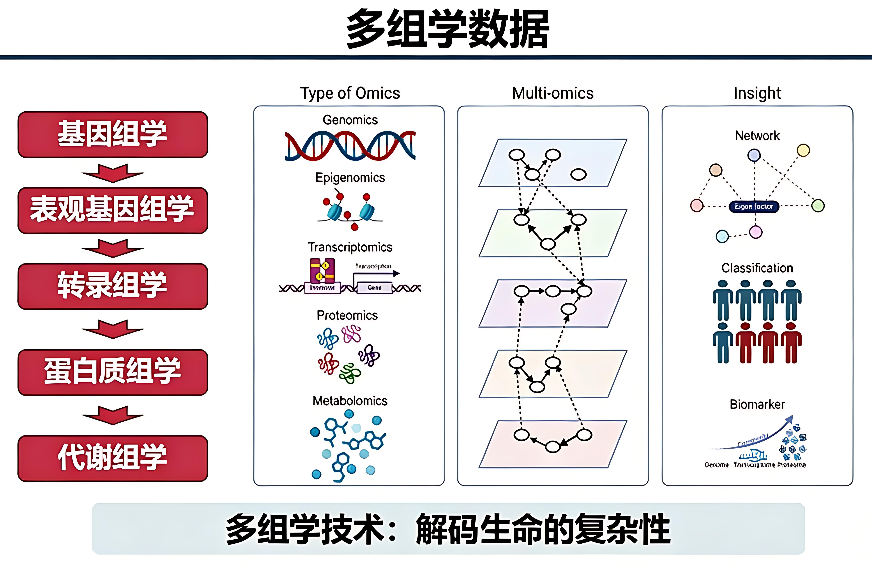
\includegraphics[width=\textwidth]{figures/c1_multiomics/01.png}
  \end{figure}
\end{frame}

\begin{frame}
  \frametitle{多组学 | 单细胞多组学}
  \begin{figure}
    \centering
    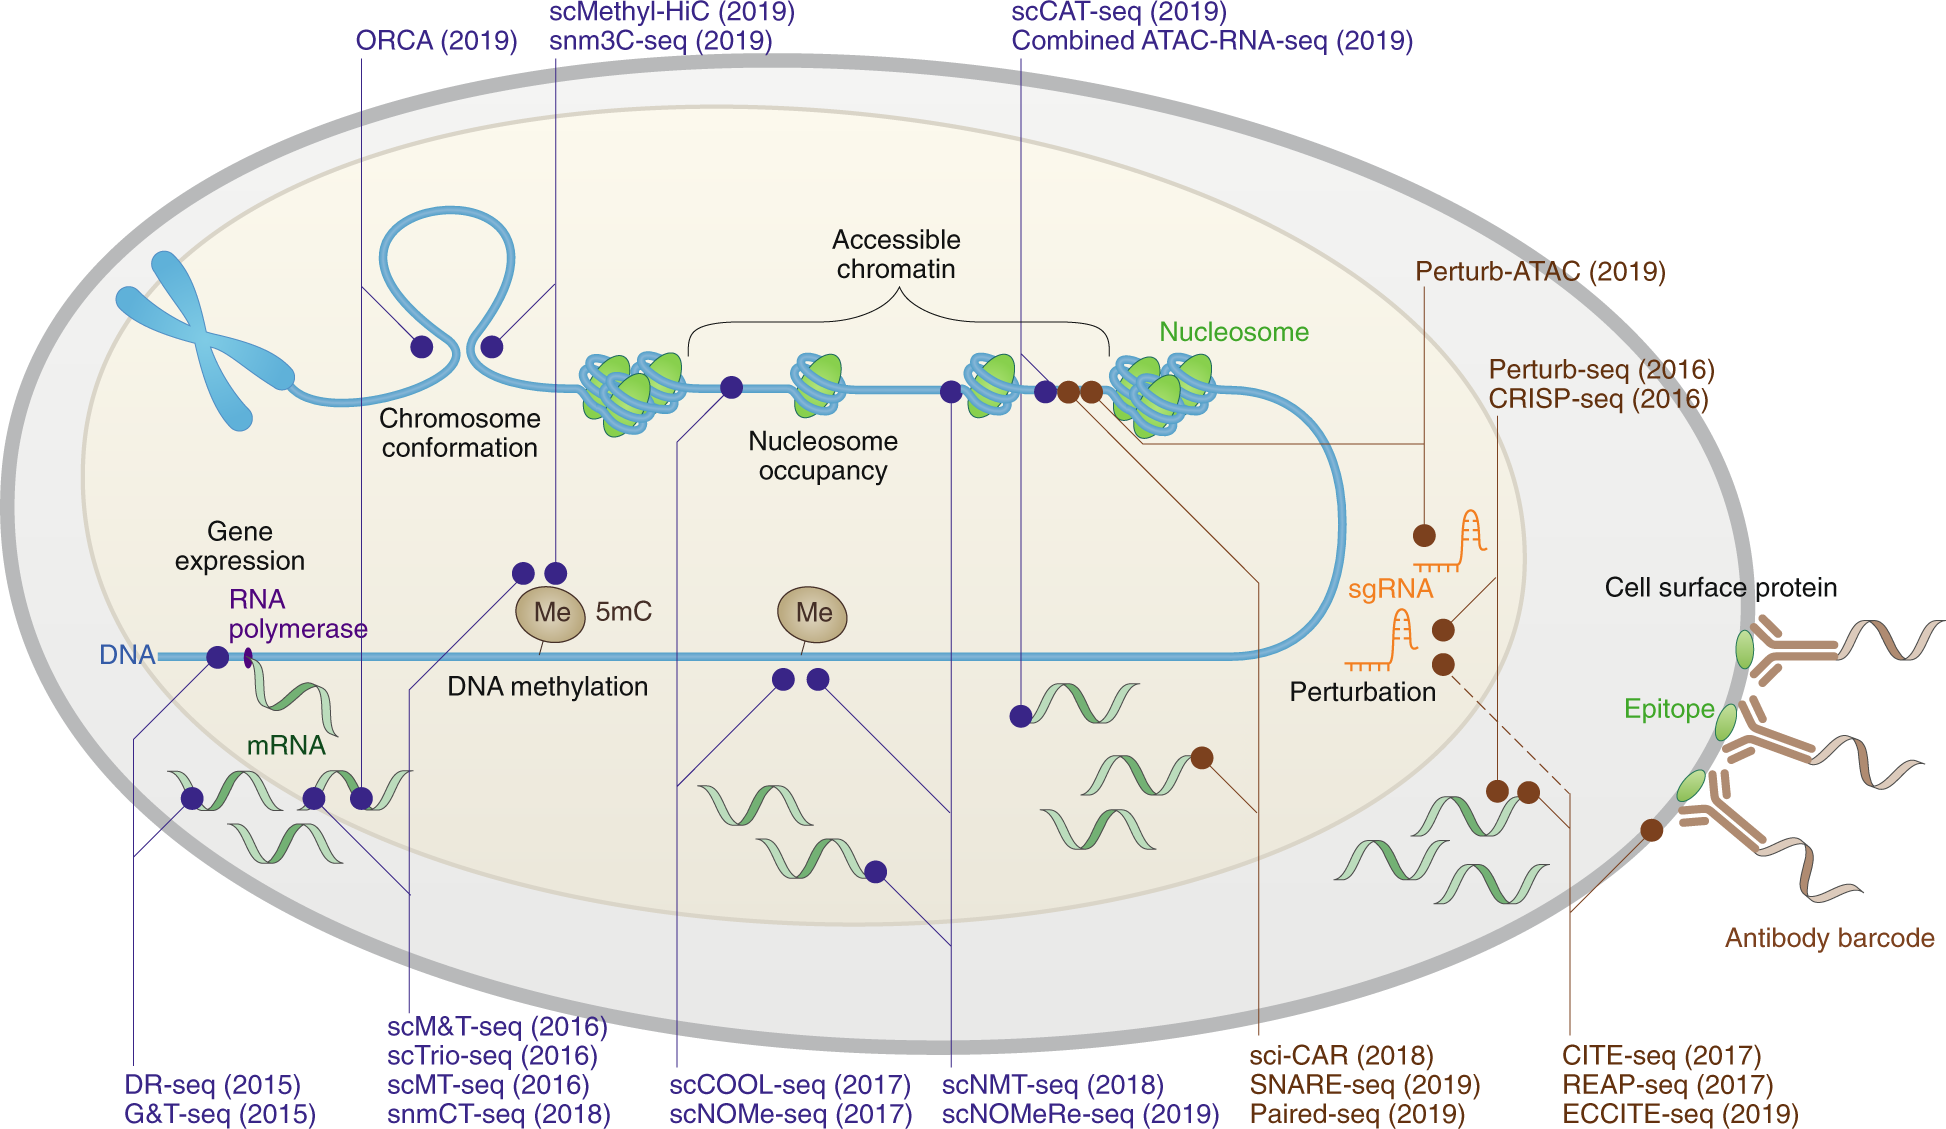
\includegraphics[width=\textwidth]{figures/c1_multiomics/scomics.png}
  \end{figure}
\end{frame}

\begin{frame}
  \frametitle{多组学 | 基因组}
  \begin{block}{基因组}
      基因组（Genome）是指生命体内包含的所有 DNA 分子，主要研究内容包括生殖细胞和体细胞的点突变、结构变异、重排突变等。
  \end{block}
  \begin{block}{常用技术}
      \begin{itemize}
          \item 在群体水平，全基因组关联分析（Genome-wide associated studies, GWAS）通过病例-对照样本的基因组学数据对比分析获得疾病相关的靶点。
          \item 在个体水平，全基因组测序（WGS）用于诊断和治疗。
          \item 外显子组测序（WES）技术通过特异捕获外显子区域 DNA 序列进行测序，成本明显低于全基因组测序的同时也能有效地检测疾病相关基因。
      \end{itemize}
  \end{block}
\end{frame}

\begin{frame}
  \frametitle{多组学 | 基因组}
  \begin{figure}
    \centering
    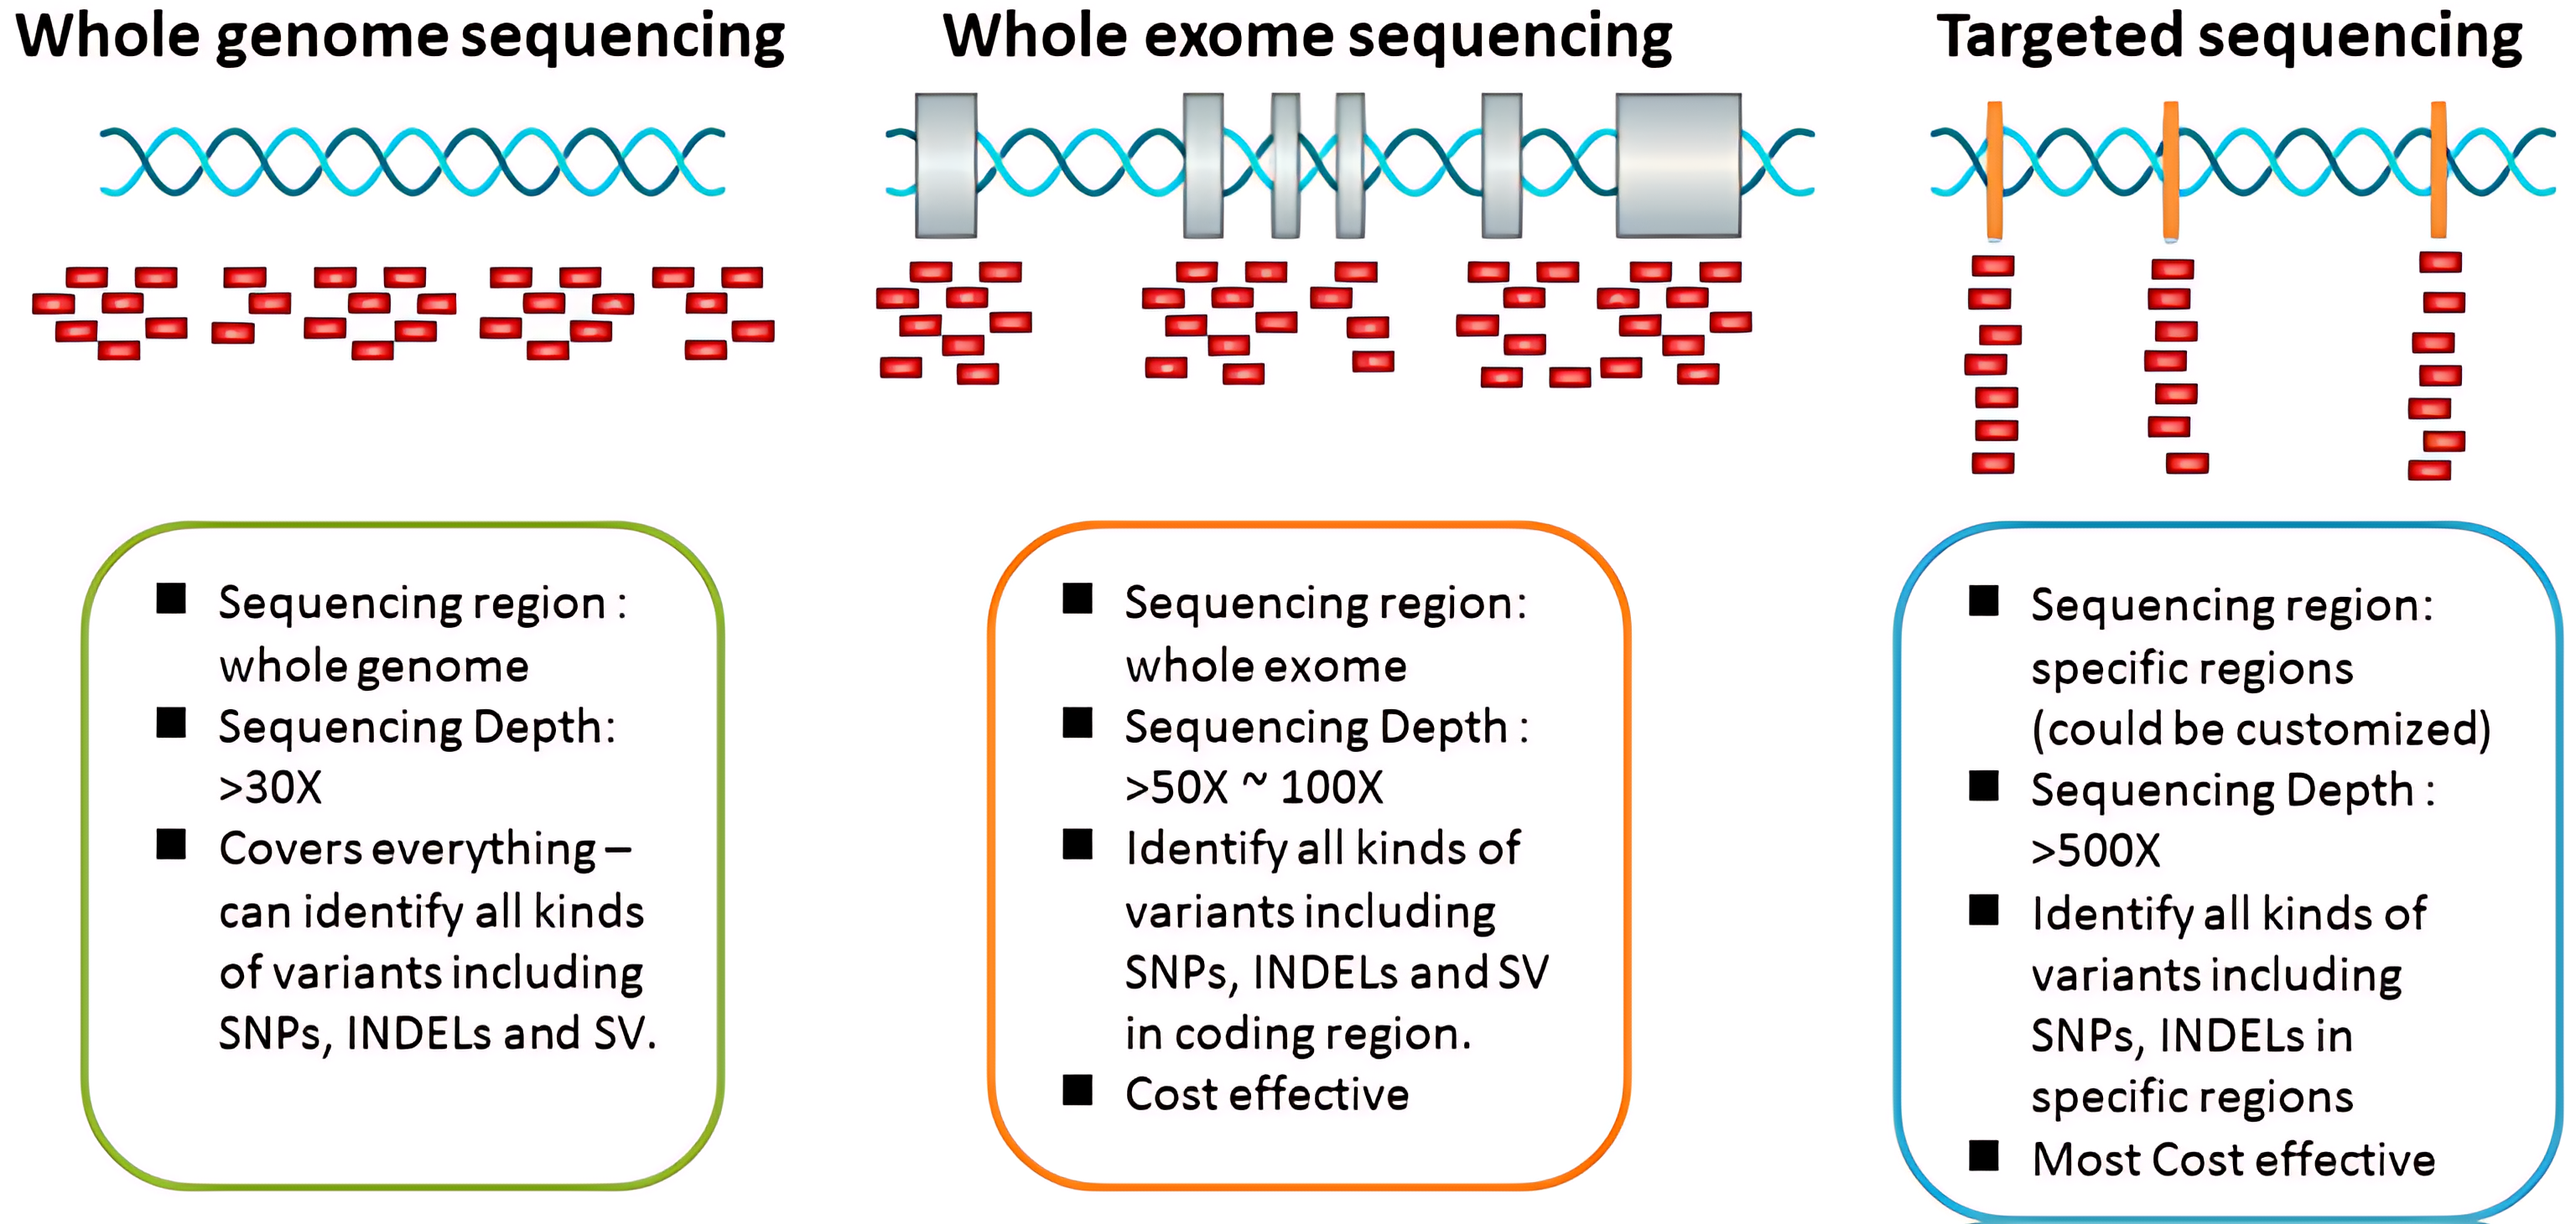
\includegraphics[width=\textwidth]{figures/c1_multiomics/wgswes.png}
  \end{figure}
\end{frame}

\begin{frame}
  \frametitle{多组学 | 基因组}
  \begin{figure}
    \centering
    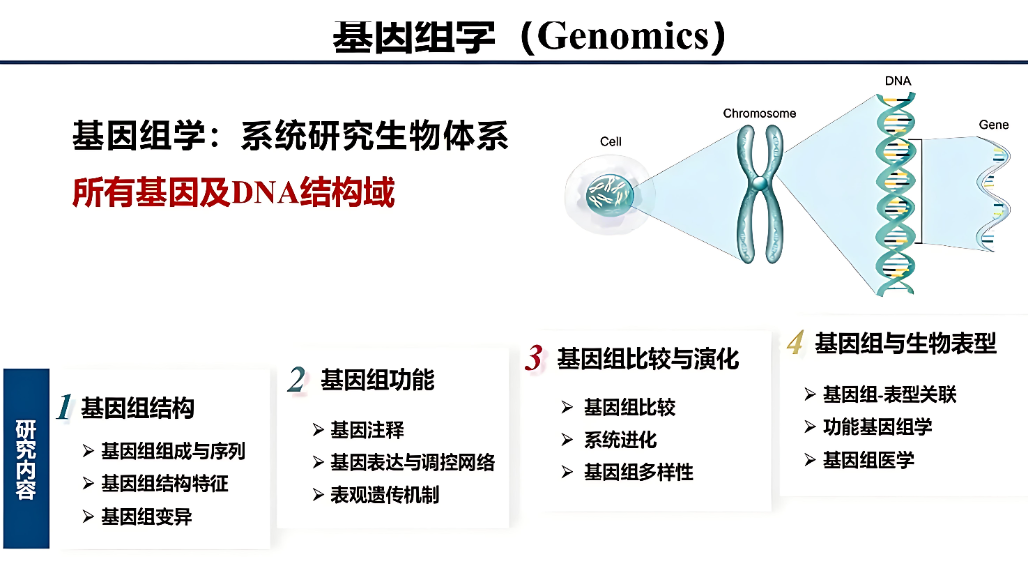
\includegraphics[width=\textwidth]{figures/c1_multiomics/02.png}
  \end{figure}
\end{frame}

\begin{frame}
  \frametitle{多组学 | 表观基因组}
  \begin{block}{表观基因组}
      \begin{itemize}
          \item \alert{表观遗传}是指 DNA 序列不发生变化，但基因表达却发生了可遗传性的改变，并且这种改变在发育和细胞增殖过程中能稳定地传递。
          \item \alert{表观基因组（Epigenome）} 主要包括 DNA 甲基化、组蛋白修饰和基因组印记等。
      \end{itemize}
  \end{block}
  \begin{figure}
    \centering
    \includegraphics[width=0.8\textwidth]{figures/c1_multiomics/epig.png}
  \end{figure}
\end{frame}

\begin{frame}
  \frametitle{多组学 | 表观基因组}
  \begin{figure}
    \centering
    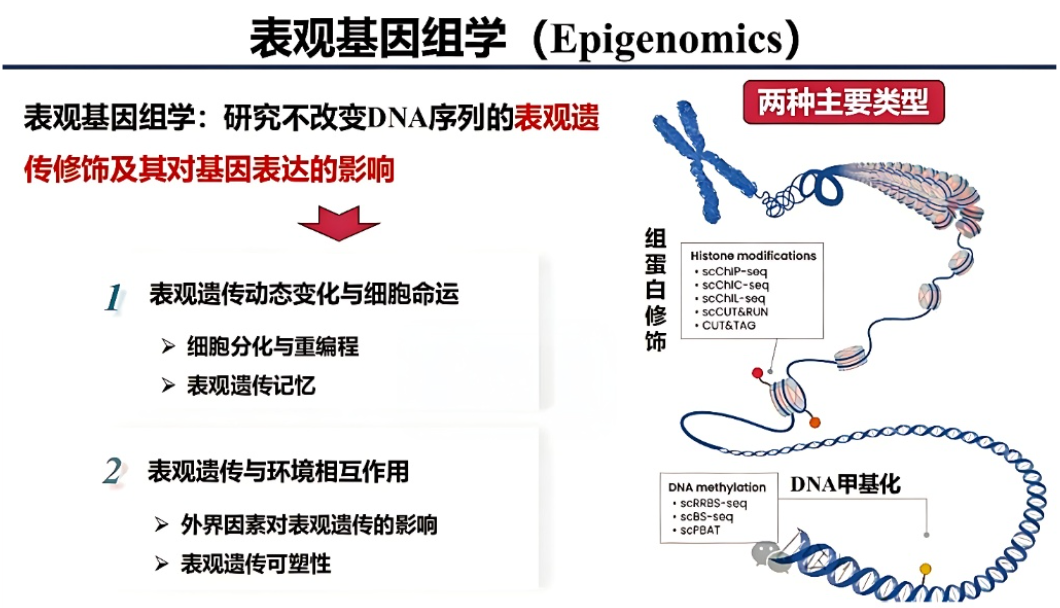
\includegraphics[width=\textwidth]{figures/c1_multiomics/03.png}
  \end{figure}
\end{frame}

\begin{frame}
  \frametitle{多组学 | 表观基因组}
  \begin{figure}
    \centering
    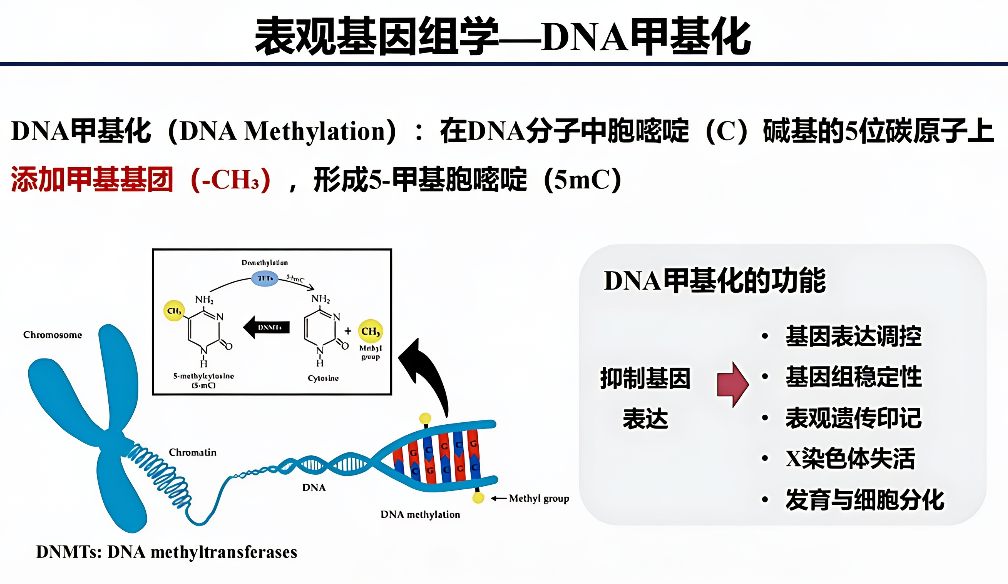
\includegraphics[width=\textwidth]{figures/c1_multiomics/04.png}
  \end{figure}
\end{frame}

\begin{frame}
  \frametitle{多组学 | 表观基因组}
  \begin{figure}
    \centering
    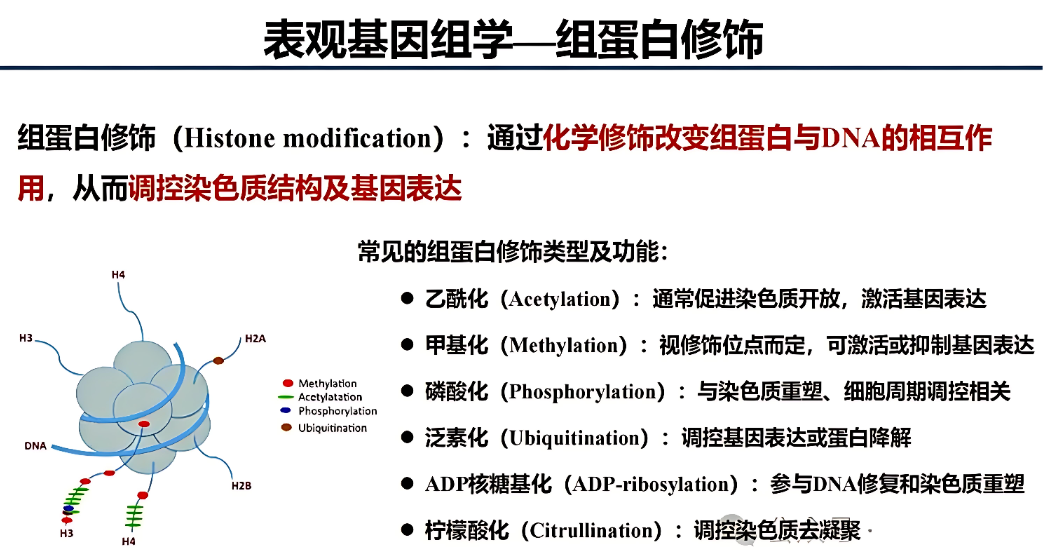
\includegraphics[width=\textwidth]{figures/c1_multiomics/05.png}
  \end{figure}
\end{frame}

\begin{frame}
  \frametitle{多组学 | 三维基因组}
  \begin{block}{三维基因组}
      \alert{三维基因组学（3D genomics）} 是一门研究基因组三维空间结构与功能的新兴学科，主要研究基因组序列在细胞核内的三维空间构象，及其对 DNA 复制、DNA 重组、基因表达调控等生物过程的生物学效应。
  \end{block}
  \begin{figure}
    \centering
    \includegraphics[width=\textwidth]{figures/c1_multiomics/3dg.png}
  \end{figure}
\end{frame}

\begin{frame}
  \frametitle{多组学 | 转录组}
\begin{columns}
    \column{0.4\textwidth}
    \begin{block}{转录组}
        \alert{转录组（Transcriptome）} 是特定组织或细胞在某一发育阶段或功能状态下转录生成的所有 RNA 的集合，包括编码蛋白的 mRNA 和各种非编码 RNA（如 microRNA、lncRNA、circRNAs 等）。
    \end{block}
    \column{0.5\textwidth}
  \begin{figure}
    \centering
    \includegraphics[width=0.8\textwidth]{figures/c1_multiomics/tx.png}
  \end{figure}
\end{columns}
\end{frame}

\begin{frame}
  \frametitle{多组学 | 转录组}
  \begin{figure}
    \centering
    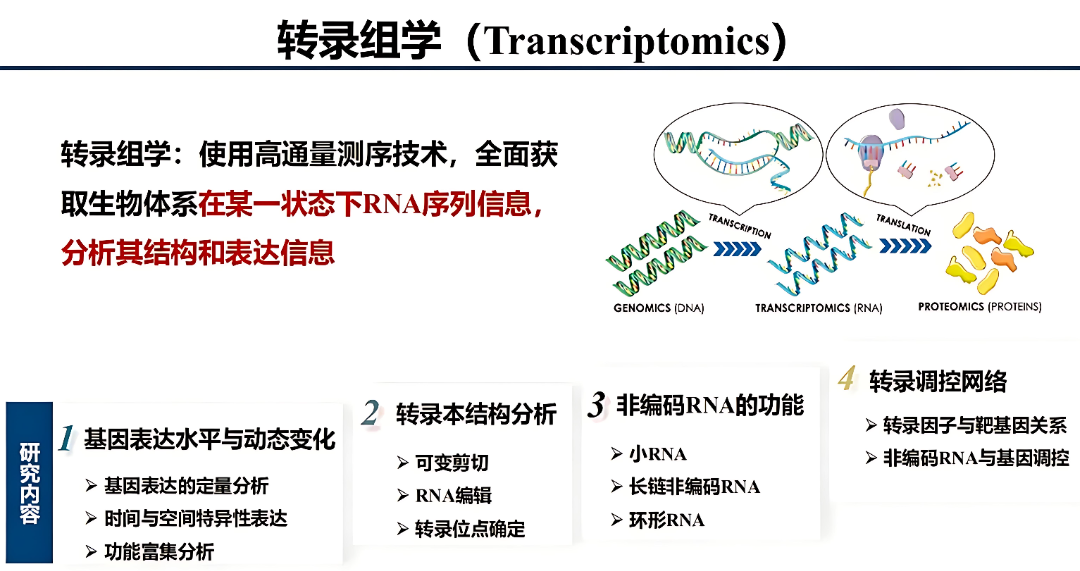
\includegraphics[width=\textwidth]{figures/c1_multiomics/06.png}
  \end{figure}
\end{frame}

\begin{frame}
  \frametitle{多组学 | 转录组}
  \begin{figure}
    \centering
    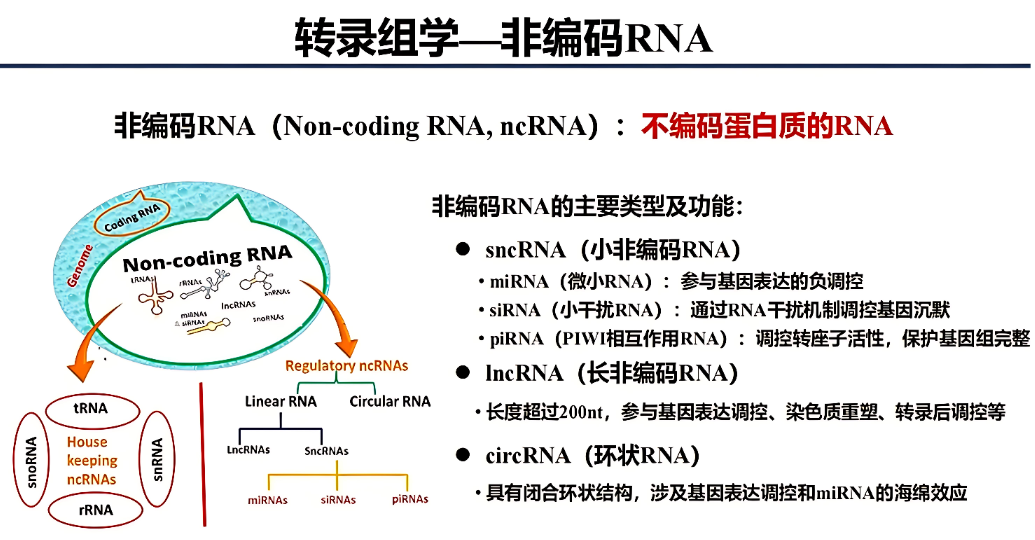
\includegraphics[width=\textwidth]{figures/c1_multiomics/07.png}
  \end{figure}
\end{frame}

\begin{frame}
  \frametitle{多组学 | 转录组}
  \begin{figure}
    \centering
    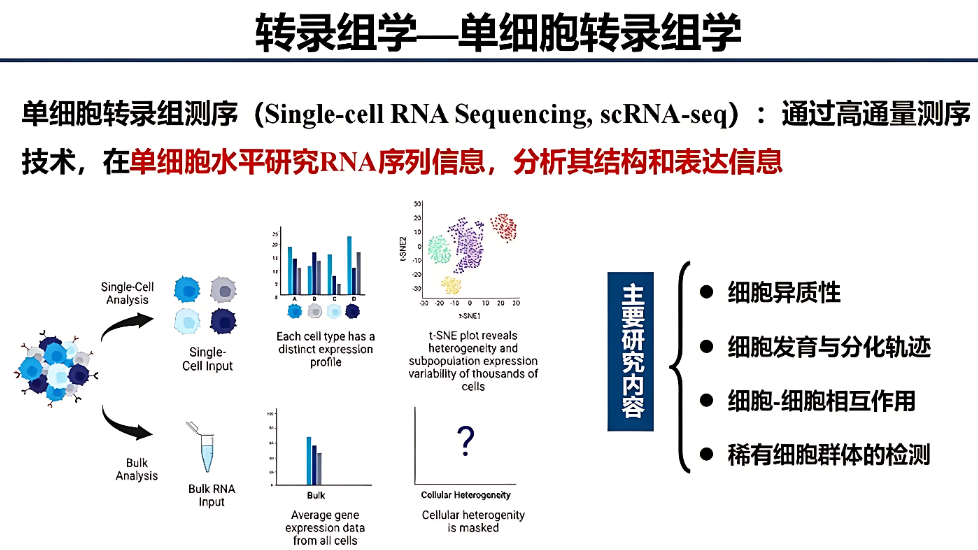
\includegraphics[width=\textwidth]{figures/c1_multiomics/08.png}
  \end{figure}
\end{frame}

\begin{frame}
  \frametitle{多组学 | 转录组}
  \begin{figure}
    \centering
    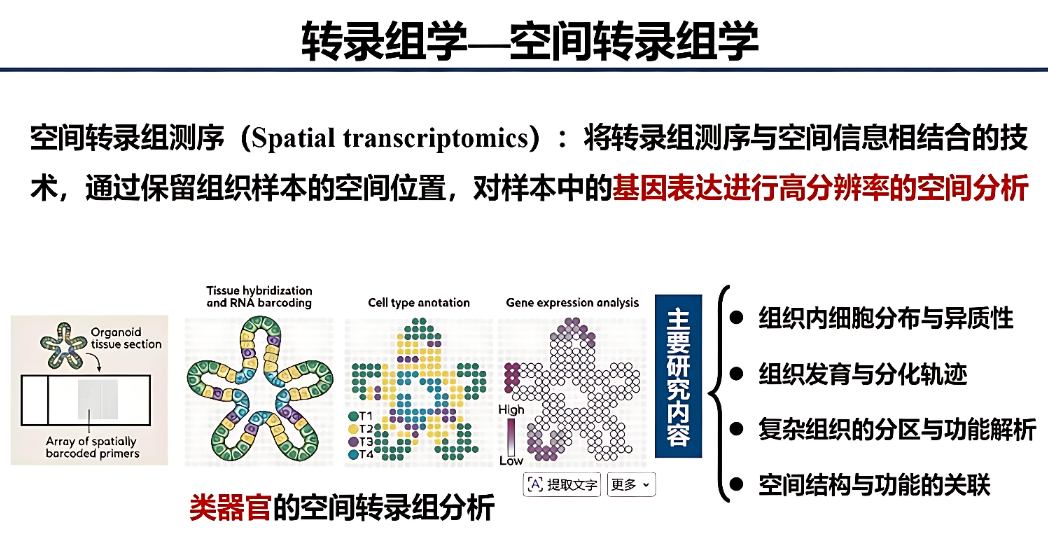
\includegraphics[width=\textwidth]{figures/c1_multiomics/09.png}
  \end{figure}
\end{frame}

\begin{frame}
  \frametitle{多组学 | 表观转录组}
  \begin{block}{表观转录组}
      \begin{itemize}
          \item \alert{表观转录组（Epitranscriptome）} 是指细胞 RNA 转录后修饰产生的生物体细胞变化。
          \item \alert{RNA修饰（RNA modification）} 指发生在 RNA 上的各种修饰形式，是转录后水平的一类调控方式，因其可逆变化与动态调控受到越来越多的关注。
      \end{itemize}
  \end{block}
  \begin{figure}
    \centering
    \includegraphics[width=0.6\textwidth]{figures/c1_multiomics/rnam.png}
  \end{figure}
\end{frame}

\begin{frame}
  \frametitle{多组学 | 蛋白质组}
  \begin{figure}
    \centering
    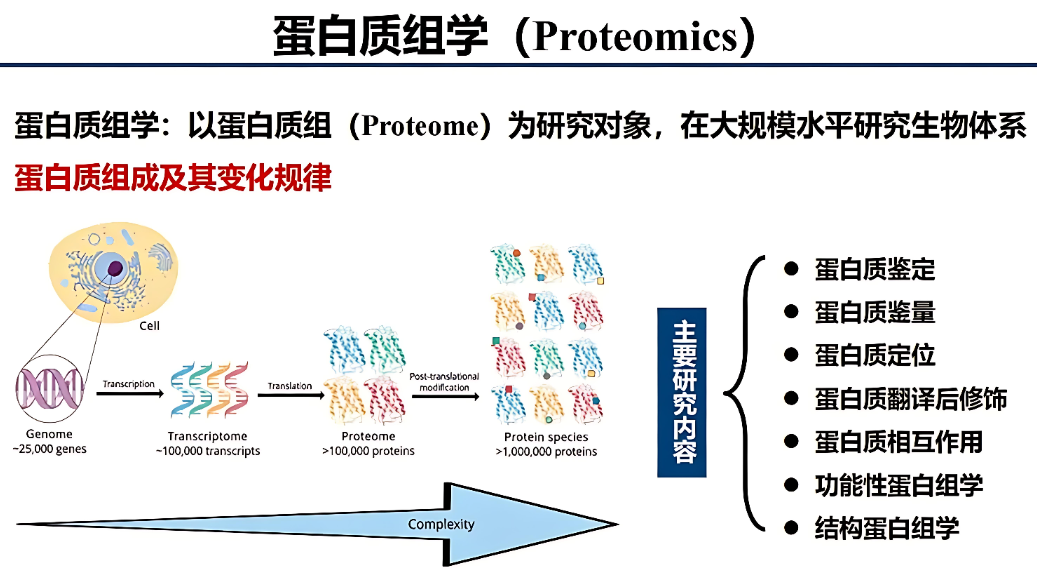
\includegraphics[width=\textwidth]{figures/c1_multiomics/10.png}
  \end{figure}
\end{frame}

\begin{frame}
  \frametitle{多组学 | 代谢组}
  \begin{figure}
    \centering
    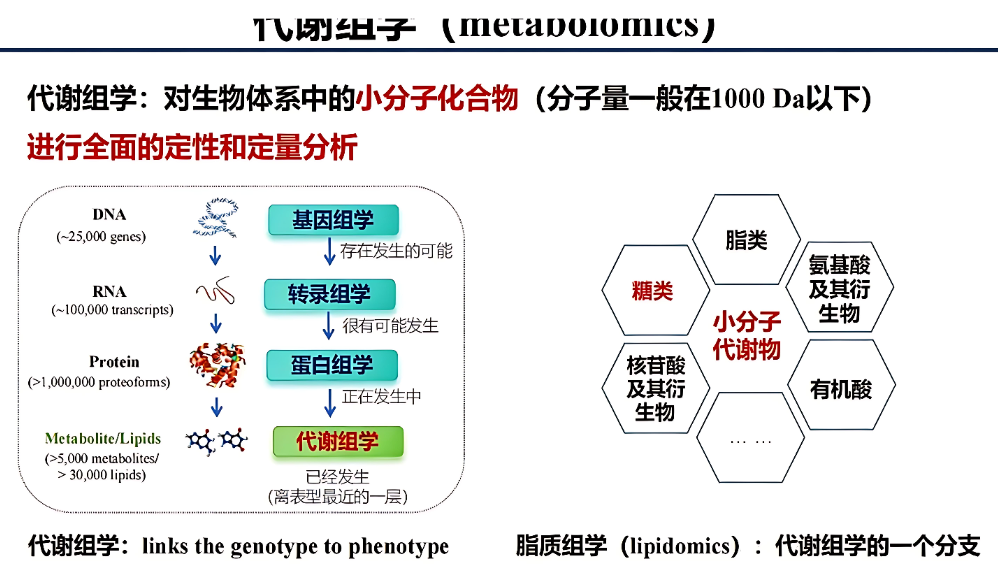
\includegraphics[width=\textwidth]{figures/c1_multiomics/11.png}
  \end{figure}
\end{frame}

\begin{frame}
  \frametitle{多组学 | 代谢组}
  \begin{figure}
    \centering
    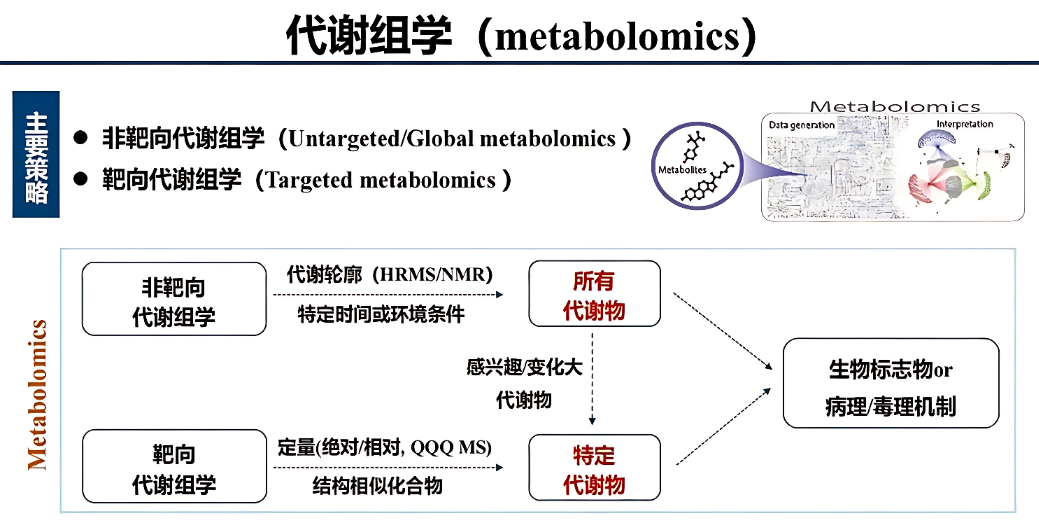
\includegraphics[width=\textwidth]{figures/c1_multiomics/12.png}
  \end{figure}
\end{frame}

\begin{frame}
  \frametitle{多组学 | 数据整合分析}
\begin{columns}
    \column{0.4\textwidth}
    \begin{block}{多组学数据整合分析}
        多组学数据整合分析的首要步骤是对不同来源的数据进行标准化处理，然后通过比较建立不同组学数据之间的关联性和差异性，进而根据这种内在联系在不同层次对候选疾病因子进行筛选过滤，最终目标是对疾病的发生过程建立定量模型，通过模拟仿真等手段预测候选疾病因子的作用，通过改变因子的水平预测治疗效果等。
    \end{block}
    \column{0.55\textwidth}
  \begin{figure}
    \centering
    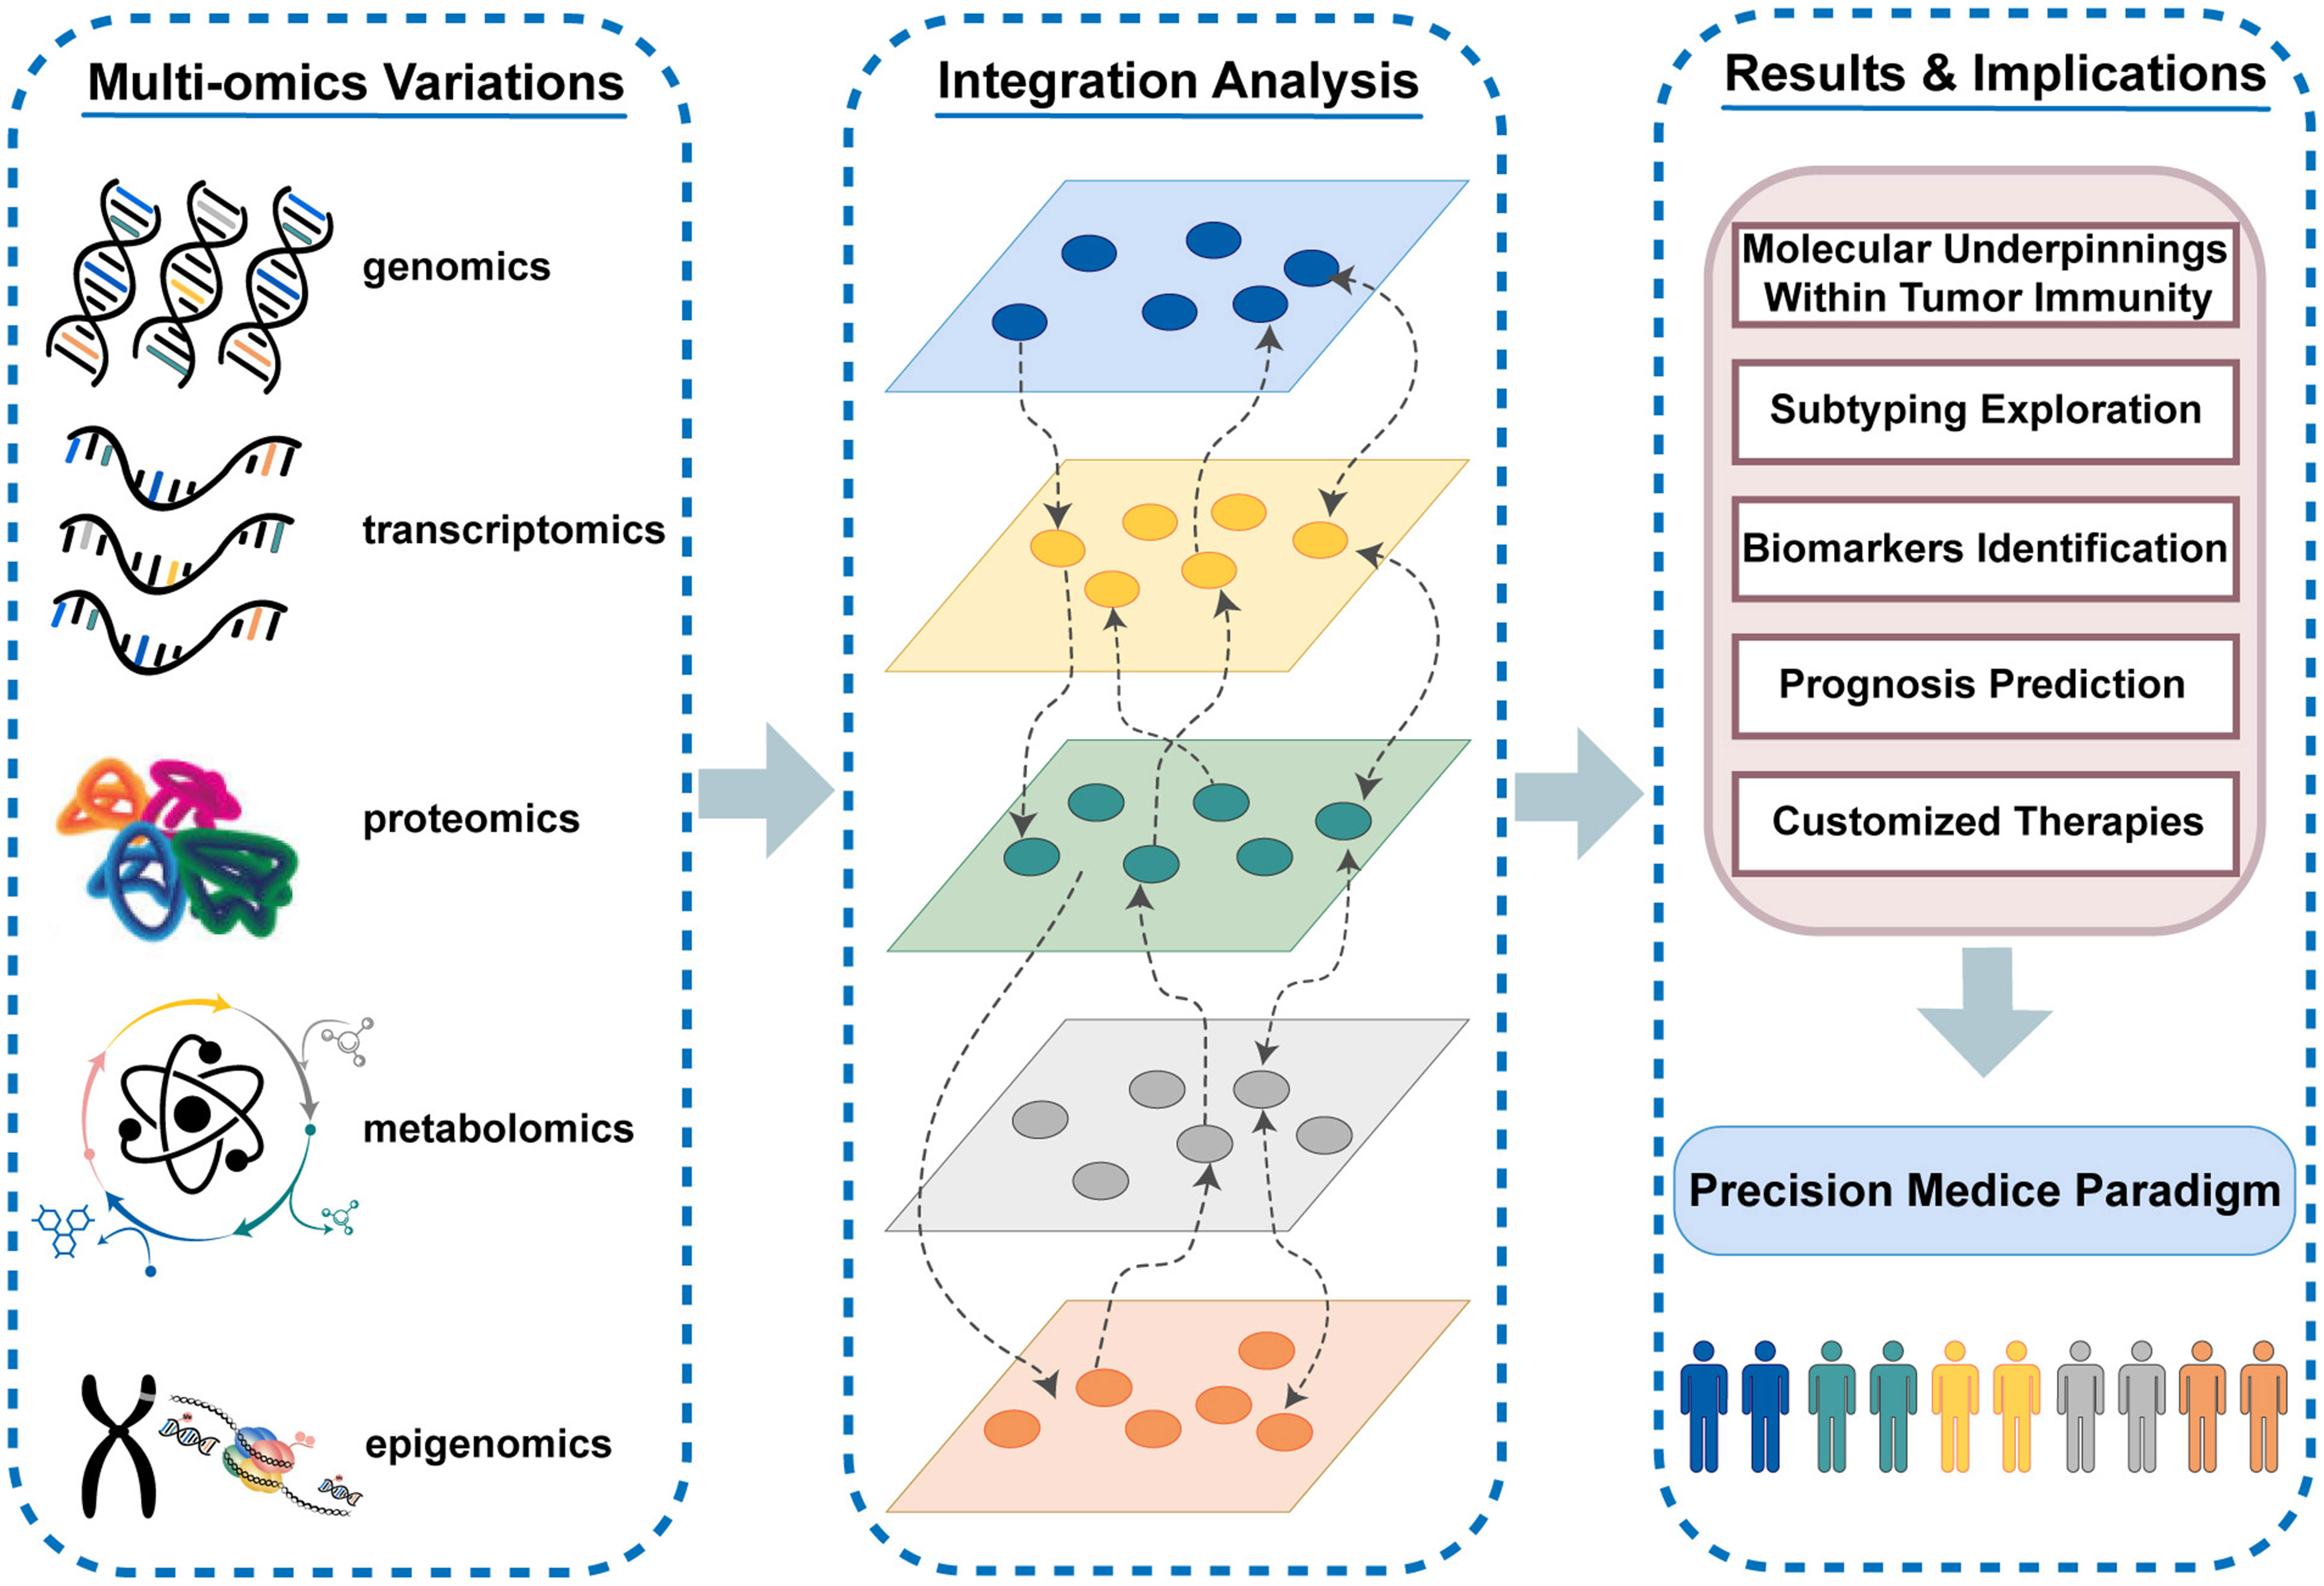
\includegraphics[width=\textwidth]{figures/c1_multiomics/integrate.png}
  \end{figure}
\end{columns}
\end{frame}

\begin{frame}
  \frametitle{多组学 | 挑战}
  \begin{figure}
    \centering
    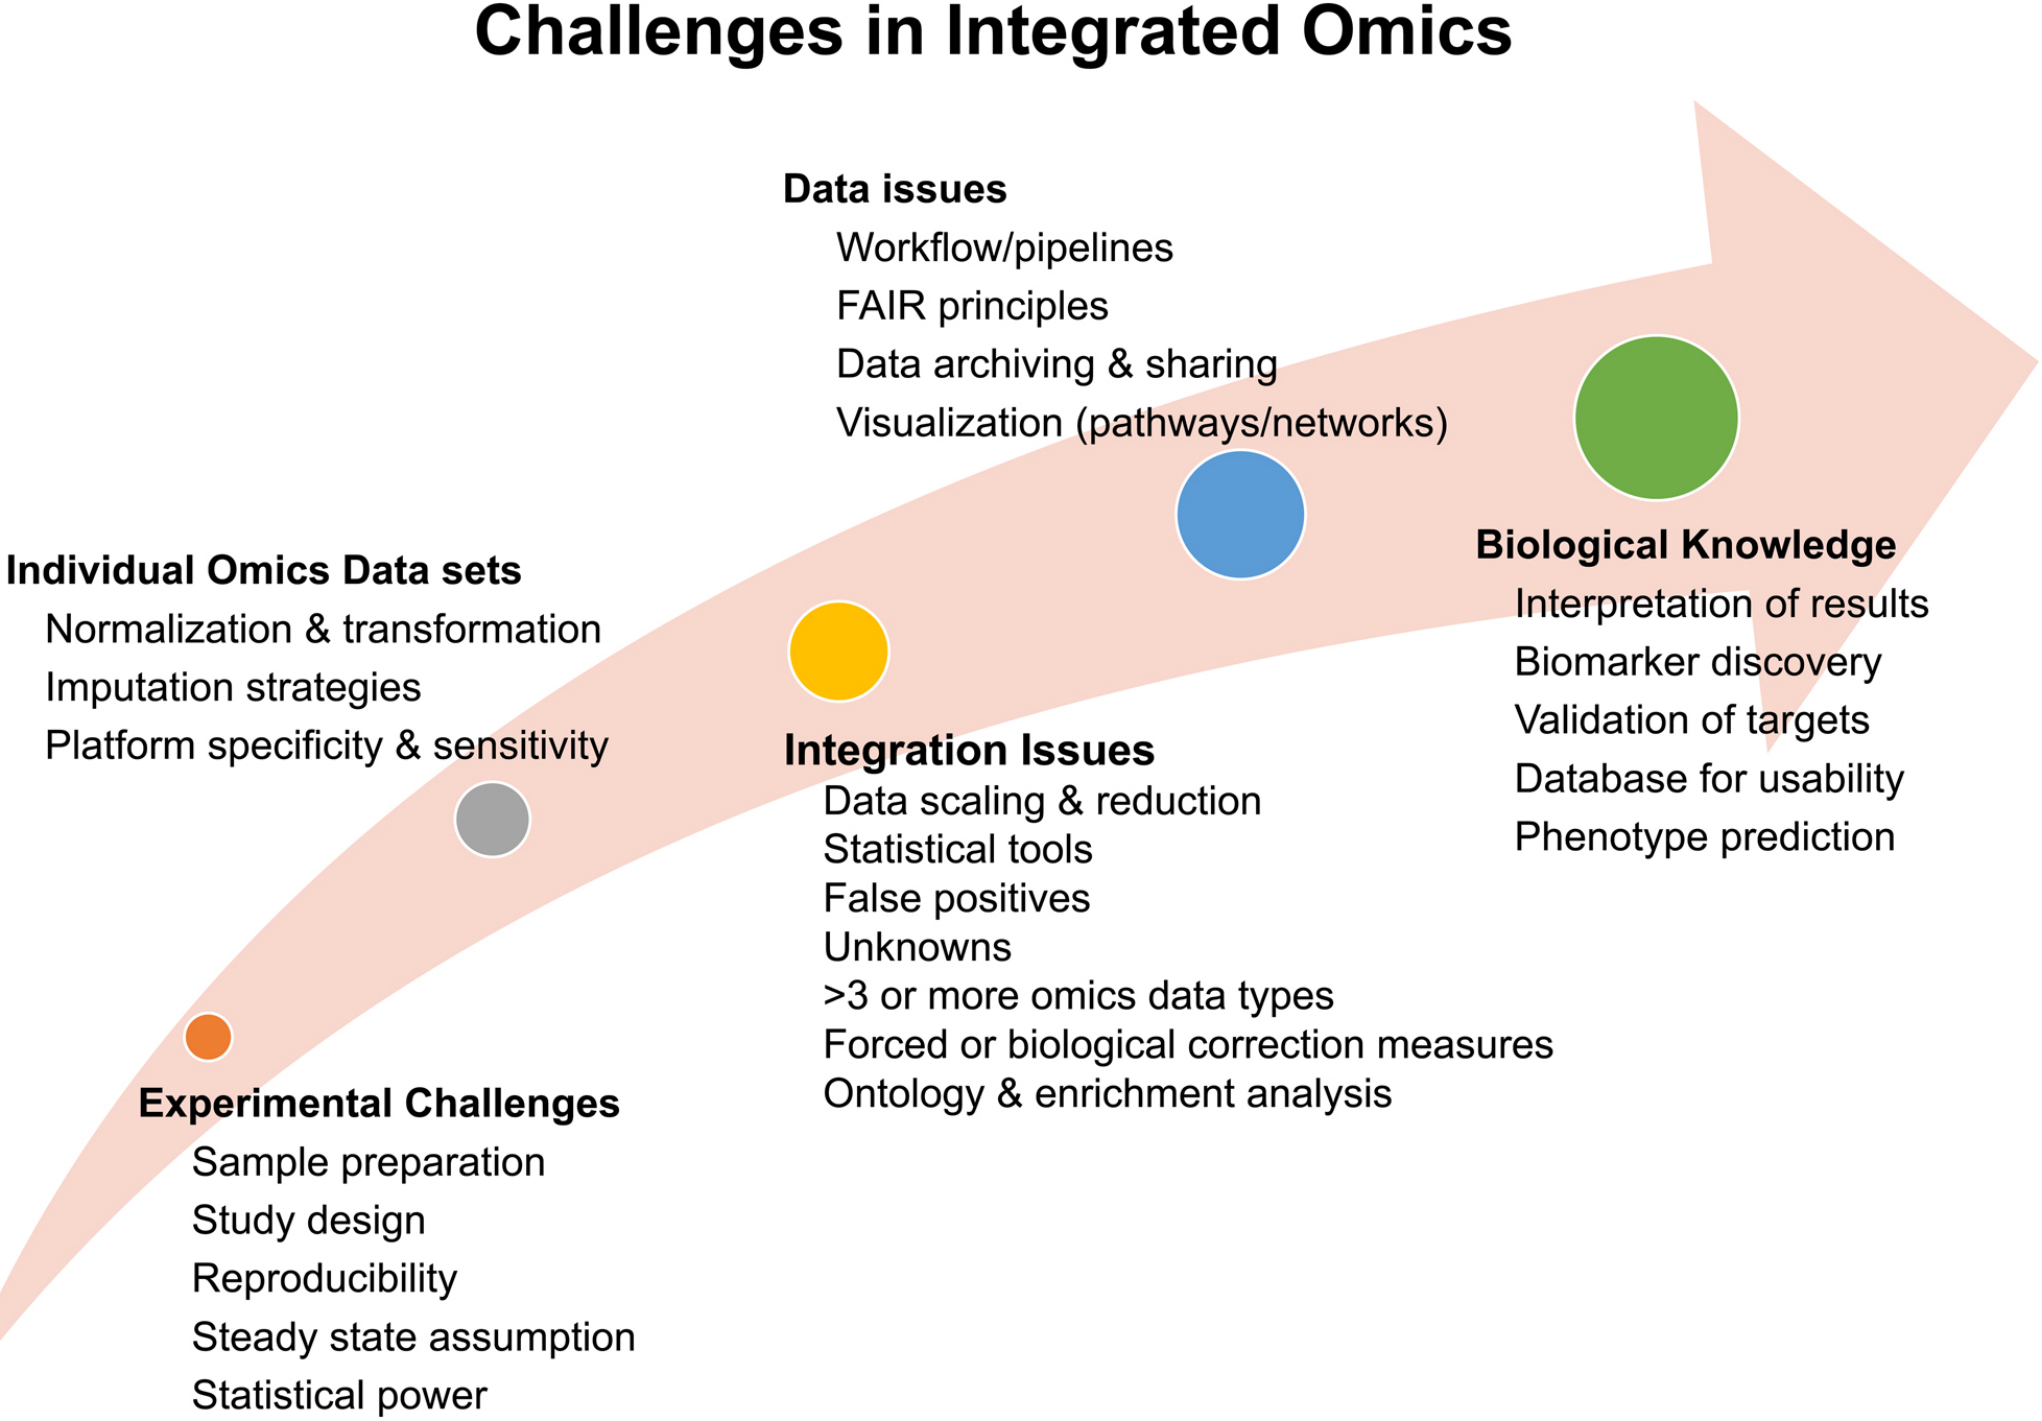
\includegraphics[width=0.9\textwidth]{figures/c1_multiomics/challenge.png}
  \end{figure}
\end{frame}

\begin{frame}
  \frametitle{多组学 | 机器学习}
  \begin{figure}
    \centering
    \includegraphics[width=\textwidth]{figures/c1_multiomics/ml.png}
  \end{figure}
\end{frame}

\begin{frame}
  \frametitle{多组学 | AI}
  \begin{figure}
    \centering
    \includegraphics[width=0.75\textwidth]{figures/c1_multiomics/ai_2.png}
  \end{figure}
\end{frame}

